\begin{figure}[htbp]
    \centering
    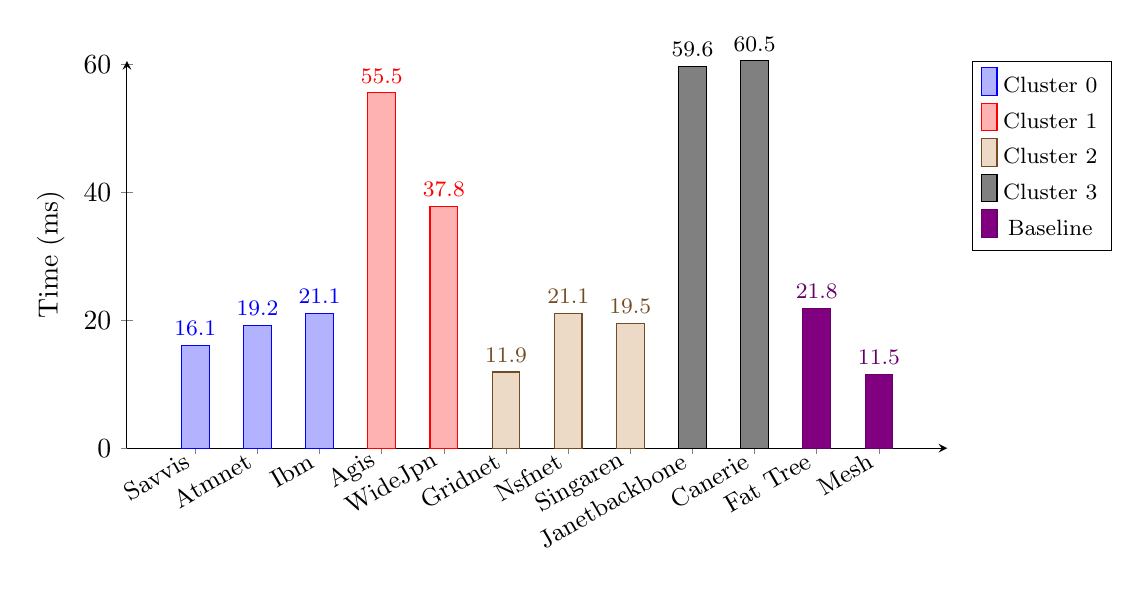
\begin{tikzpicture}
        %xmin, ymin, xmax, ymax
    \begin{axis}[
        ybar, bar width=10pt,
        axis lines=left, ylabel={Time (ms)}, ymin=0,
        enlarge x limits=0.1,
        width=12cm, height=6.5cm, 
        scaled y ticks=false,
        yticklabel style={/pgf/number format/fixed},
        symbolic x coords={Savvis, Atmnet, Ibm, Agis, WideJpn, Gridnet, Nsfnet, Singaren, Janetbackbone, Canerie, Fat Tree, Mesh},
        xtick={Savvis, Atmnet, Ibm, Agis, WideJpn, Gridnet, Nsfnet, Singaren, Janetbackbone, Canerie, Fat Tree, Mesh},
        nodes near coords,
        nodes near coords style={
            font=\footnotesize,
        },
        x tick label style={rotate=30, anchor=east, font=\small},
        bar shift=0pt,
        legend image code/.code={
            \draw (0cm,-0.1cm) rectangle (0.2cm,0.25cm); },
        legend style={font=\footnotesize},
        legend pos=outer north east,
    ]
    
        \addplot coordinates{
            (Savvis, 16.1)
            (Atmnet, 19.2)
            (Ibm, 21.1)
        };
        \addplot coordinates {
            (Agis, 55.5)
            (WideJpn, 37.8)
        };
        \addplot coordinates{
            (Gridnet, 11.9)
            (Nsfnet, 21.1)
            (Singaren, 19.5)
        };
        \addplot coordinates {
            (Janetbackbone, 59.6)
            (Canerie, 60.5)
        };
        \addplot coordinates {
            (Fat Tree, 21.8)
            (Mesh, 11.5)
        };

        \legend{Cluster 0, Cluster 1, Cluster 2, Cluster 3, Baseline}
    \end{axis}
    \end{tikzpicture}
\end{figure}
